\section{Online Adaptation}
\label{sec:hyp_test}
The online phase of the algorithm we create a scene graph $\mathcal{G} = \{V,E\}$, this graph at a selected vertex and update the action parametrization by updating the feature weights by gradient descent in feature space. The online phase of the algorithm has three stages; a supervised classification phase, a data association phase and an online gradient update phase. The three phases are discussed in detail in the sections below.
\subsection{Supervised Classification}
When a scene is presented to the agent (robot) in the form of an rgb image and corresponding point cloud is used to construct a scene graph $\mathcal{G}$. We first pre-process the point cloud to look for euclidean clusters supported by some dominant plane in the image. Once these clusters have been detected we project them back on to the image to get the corresponding image patches.

To construct the scene graph we oversegment these image patches in to superpixels using the graph based segmentation approach described in (\cite{Javidi12_Journal} TODO: Fix Citation). We then construct the scene graph by analyzing the nearest neighbours of each superpixel segment. Every vertex $V_i$ of the graph $\mathcal{G}$ would be correspond to a superpixel and the edges $E_j$ would be be drawn between superpixels touching each other. From such a respresentation the notion of rigid and dynamic edges are readily apparent as rigid edges are those edges that connect superpixels on the same object and dynamic edges are those edges that connect superpixels between two objects that are touching or in close proximity to each other. This is illustrated in the figure below Fig \ref{fig:scene_graph}.

\begin{figure}[ht!]
	\centering
	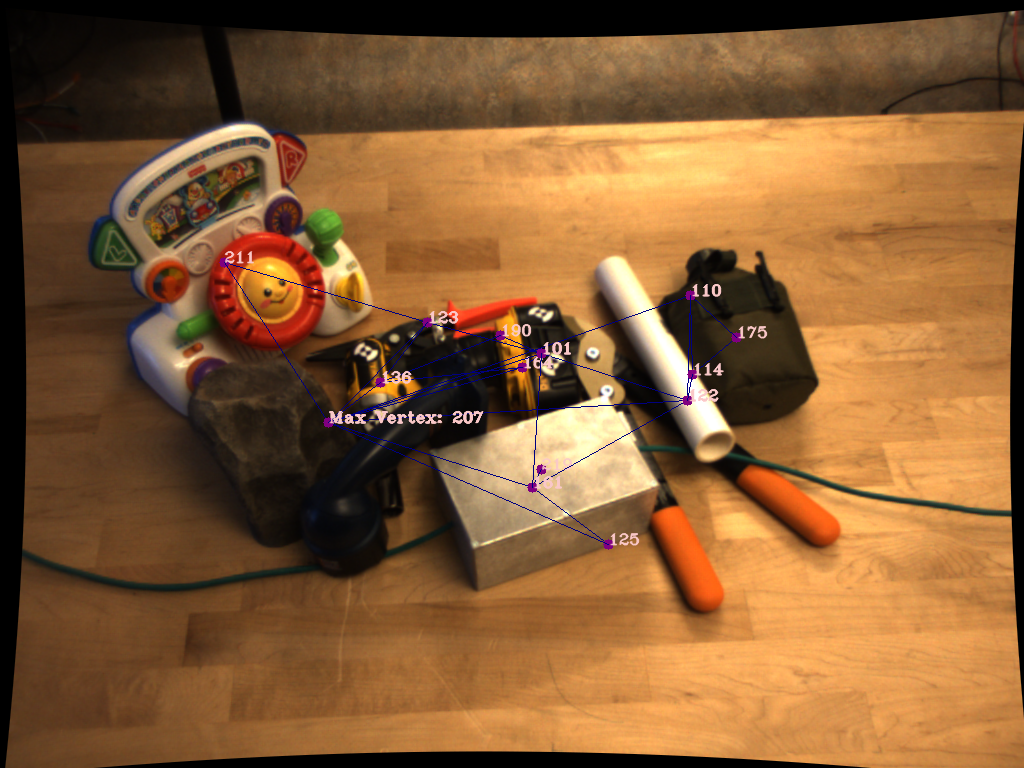
\includegraphics[width=\linewidth]{figs/full_graph.png}
	\caption{Illustrates the scene graph construction from a set of objects on a table}
	\label{fig:scene_graph}
\end{figure}

Once we generate the scene graph $\mathcal{G}$, we compute the set of features described in Section \ref{sec:lfd} for the vertex of maximum degree $V_{max}$ in the graph. The intuition for only attempting to manipulate the Vertex of maximum degree is that it is connected the most number of other vertices hence manipulating this vertex can impact the graph adjacency matrix more severly than any other node.

Once we compute the features for the max degree vertex $V_{max}$ we use the weights computed using the max entropy learner in the offline learning phase discussed in Section \ref{sec:lfd}. Using these weights we select the best action to execute by sampling the best action from a gibbs distribution as shown below.

\[
a_t = \max(\frac{\exp^{w^Tf(x)}}{ \sum_b\exp^{w^Tf(x)}})\\
\]

Once we generate the action to be executed we execute the action $a_t$ and observe the corresponding reward $R_t$. Here $t$ is the current time step and $f(x)$ is the feature function.

\subsection{Data Association}
Once the action is executed we track the vertices of the scene graph $\mathcal{G}_t$ using optical flow. The positions of the vertices of the graph are updated using the Gunnar Farnebaack Optical Flow algorithm (\cite{Javidi12_Journal} TODO: Cite Gunnars' ICPR 2000 paper) to obtain the predicted scene graph update $\tilde{\mathcal{G}}_{t+1}$. Once the vertices in the graph are updated to get the predicted graph $\tilde{\mathcal{G}}_{t+1}$, the predicted graph is matched with the observed scene graph $\hat{\mathcal{G}}_{t+1}$ to get the actual scene graph $\mathcal{G}_{t+1}$. The graph matching is accomplished by measuring the Bhattacharya distance given by

\[
D_B(p,q) = -\log{\sum_{x\in\mathcal{X}}\sqrt{p(x)q(x)}}\\
\]

between the appearance histograms of the vertices of each graph. Using this distance metric we are able to establish an accurate correspondence between $\tilde{\mathcal{G}}_{t+1}$ and $\hat{\mathcal{G}}_{t+1}$, to get $\mathcal{G}_{t+1}$. This correspondence matching is show below in Figure \ref{fig:correspondence}.

\begin{figure}[ht!]
	\centering
	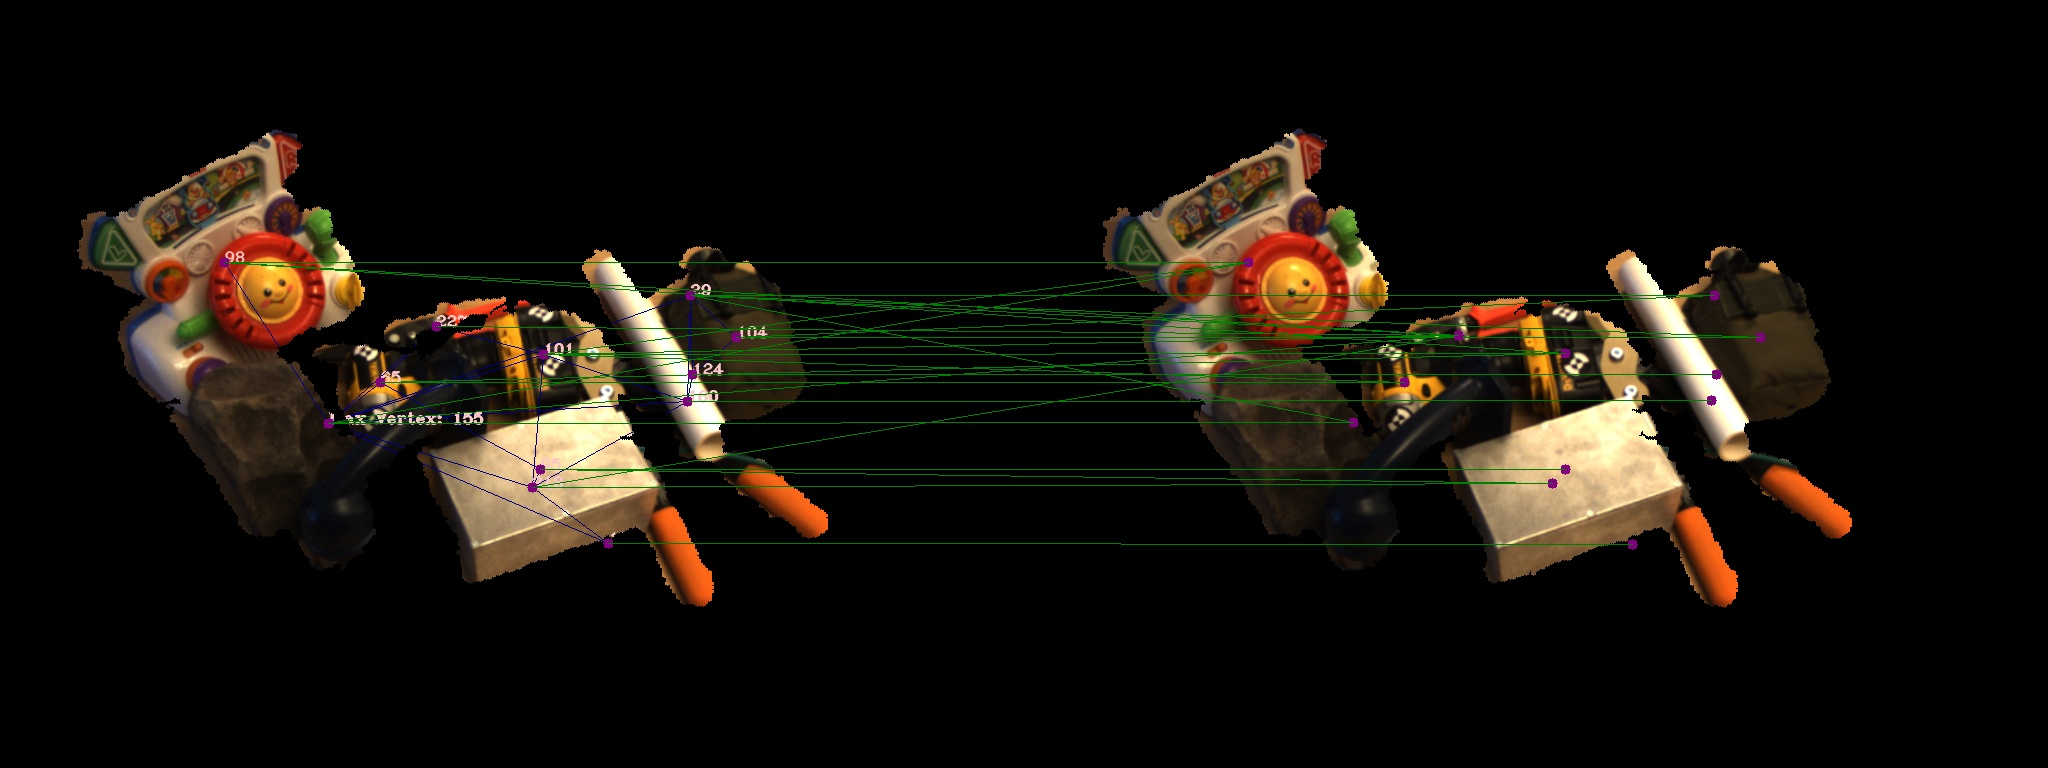
\includegraphics[width=\linewidth]{figs/correspondence.jpg}
	\caption{Show's the result of the Graph Matching algorithm after the Optical Flow update}
	\label{fig:correspondence}
\end{figure}


Once we get the updated scene graph $\mathcal{G}_{t+1}$ we perform an online policy gradient update utilizing the expected reward and the observed reward from the updated scene graph.

\subsection{Online Feature Gradient Update}
A policy gradient method is a {\bf reinforcement learning} method that directly optimizes a parametrized control policy by gradient descent. Since we use discrete actions in our approach; as opposed to performing gradient descent in policy space we peform gradient descent in feature space, thereby adapting the action selection to the current scene being observed. This is accomplished in a method similar to that employed by policy gradient approaches.

Our feature gradient also follows the gradient of the expected return where the feature weights are updated as follows.

\[
w_{k+1} = w_k + \alpha_k\bigtriangledown_w{\it J(\pi_w)}|_{w=w_k}\\
\]

where ${\it J(\pi_w)}$ the gradient on the reward is computed using regular regression

\[
\bigtriangledown_w = (\Delta W^T\Delta W)^{-1}\Delta W^T\Delta {\it J}\\
\]

The mean-subtracted reward return $\Delta {\it J}$ is obtained by subtracting the observed reward from the expected reward. The expected reward is given a function of the features weights computed using the Max Entropy learner in the offline phase. Hence the expected reward is $J(\hat{w}_k) = W^Tf(x)$. The observed reward is expected reward weighted by the variation in spectral norm of the adjacency matrix. This is given by

\[
\bar{J(w_k)} = \frac{1}{(\|A_{t+1}\| - \|A_t\|)}*\beta*J(\hat{w}_k)\\
\]

where $\beta$ is an appropriate scaling factor. The reason we use the spectral norm is because the spectral norm measures the magnitude of the largest singular value of a matrix. And to measure the similarity between two matrices we can compare their spectral norms. Hence using this logic the gradient update is performed as long as the observed adjaceny matrix and the actual adjacency matrix are different.

Once this update is performed a new action is sampled from the gibbs distribution parametrized by the updated feature weights. The actions are sampled until the variation in the spectral norm goes to zero or the feature weights top updating.
% In this section we provide a dynamic programming formulation for the single object optimization problem in (\ref{eq:sequential_optimization}). As mentioned earlier, we restrict the possible sensor poses to a discrete set $\mathcal{X}(\rho)$ of viewpoints on the viewsphere $V(\rho)$ centered at the unknown object. The state at time $t$ consists of the sensor pose $x_t \in \mathcal{X}(\rho)$ and the \textit{information state}, summarized by the sufficient statistic consisting of the probabilities for each hypothesis:
% \[
% p_i(t) = \mathbb{P}(H_i \mid Z_1=z_1,\ldots,Z_t=z_t, x_{0:t}) \in [0,1],
% \]
% where $z_{1:t}$ are the observations from the vocabulary tree. Suppose that at time $t$ the state is $(x_t,p(t))$ and the sensor decides to continue observing by moving to a new viewpoint $x_{t+1}\in\mathcal{X}(\rho)$. The new observation $z_{t+1}$ is used to update the probabilities of the hypotheses according to Bayes' rule:
% \begin{align*}
% p(t+1) &= T(p(t),x_{t+1},z_{t+1}), \text{ with $i$th component:}\\
% p_i(t+1) &= \mathbb{P}(H_i \mid z_{1:(t+1)},x_{0:(t+1)})\\
% &=\frac{\mathbb{P}(Z_{t+1} = z_{t+1} \mid x_{t+1}, H_i)\mathbb{P}(H_i \mid z_{1:t}, x_{0:t})}{\mathbb{P}(Z_{t+1} = z_{t+1}\mid x_{t+1})}\\
% &=\frac{h_i^{x_{t+1}}(z_{t+1})p_i(t)}{\sum_{j=0}^{M-1} h_j^{x_{t+1}}(z_{t+1}) p_j(t) }, \quad \forall i = 0,\ldots, M-1
% \end{align*}
% using the assumption of independence of successive observations. Supposing that $\tau$ is fixed for a moment, the terminal cost of the dynamic program can be derived after the latest observation $z_\tau$ has been incorporated in the posterior:
% \begin{align*}
% J_\tau(x_\tau,p(\tau)) &= \min_{\delta \in \{0,\ldots,M-1\}} \mathbb{E}_{Y,R} \Lambda_{\delta,j^*(Y,R)} \\
% &= \min_{\delta \in \{0,\ldots,M-1\}} \sum_{j=0}^{M-1} \Lambda_{\delta,j} p_j(\tau)
% \end{align*}
% The intermediate stage costs for $t = 0,\ldots,(\tau-1)$ are:
% \begin{align*}
% J_t(x_t,p(t)) = &\min_{v \in \mathcal{X}(\rho)} \biggl\{ c(x_t, v) + \\
% &\mathbb{E}_{Z_{t+1}} J_{t+1} (v, T(p(t), v, Z_{t+1})) \biggr\}
% \end{align*}
% Letting $\tau$ be random again and $t$ go to infinity we get the following infinite-horizon dynamic programming equation:
% \begin{align}
% \label{eq:mary_hypothesis}
% J(x,p) = &\min\biggl\{ \min_{\delta \in \{0,\ldots,M-1\}} \sum_{j=0}^{M-1} \Lambda_{\delta j} p_j, \\
% &\min_{v \in \mathcal{X}(\rho)} c(x,v) + \mathbb{E}_{Z} \{J(v,T(p,v,Z))\}\biggr\},\notag
% \end{align}
% which is well-posed by Propositions 9.8 and 9.10 in \cite{Bertsekas07_SoC}. Equation (\ref{eq:mary_hypothesis}) gives an intuition about the relationship between the cost functions $c(\cdot,\cdot)$, $\Lambda_{ij}$ and the stopping time $\tau$. If at time $t$, the expected cost of making a mistake given by $\min_{\delta \in \{0,\ldots,M-1\}} \sum_{j=0}^{M-1} \Lambda_{\delta j} p_j(t)$ is smaller than the cost of taking one more measurement, the sensor stops and chooses the minimizing hypothesis; otherwise it continues measuring.
% 
% We resort to numerical approximation techniques, which work well when the state space of the problem is sufficiently small. The decision rule $\delta(\cdot)$ can be replaced by a set of sink states $A = \{a_0,\ldots,a_{M-1}\}$ such that if the sensor goes to state $a_i$, it decides on hypothesis $H_i$ and remains there for the rest of time. Then, for $s_1, s_2 \in \mathcal{X}(\rho) \cup A$ the cost of movement and the state transition function become:
% \begin{align*}
% c'(s_1,p,s_2) &= \begin{cases}
% 				c(s_1, s_2), & s_1,s_2 \in \mathcal{X}(\rho)\\
% 				\sum_{j=0}^{M-1} p_j\Lambda_{s_2,j}, & s_1 \in \mathcal{X}(\rho), s_2 \in A\\
% 				0, & s_1=s_2 \in A\\
% 				\infty, & \text{otherwise}
% 			\end{cases}\\
% T'(p(t),s_{t+1},&z_{t+1}) = \begin{cases}
% 				T(p(t),s_{t+1},z_{t+1}), & s_{t+1} \in \mathcal{X}(\rho)\\
% 				p(t), & s_{t+1} \in A
% 			\end{cases}
% \end{align*}
% We can rewrite (\ref{eq:mary_hypothesis}) into the usual Bellman optimality equation for a POMDP:
% \[
% J(s,p) = \min_{s' \in \mathcal{X}(\rho)\cup A} \biggl\{c'(s,p,s') + \mathbb{E}_Z\{J(s', T'(p,s',Z) \} \biggr\}
% \]
% We use a point-based POMDP algorithm \cite{Kurniawati08_sarsop, Ong08_sarsop}, which approximates optimally reachable belief spaces in order to solve the problem efficiently and obtain an approximate stationary policy $\hat{\mu}: \mathcal{X}(\rho)\cup A \times [0,1]^M \rightarrow \mathcal{X}(\rho)\cup A$.

%The online procedure for using $\hat{\mu}$ is summarized in Algorithm \ref{alg:alg1}.
%\begin{algorithm}[H]
%\caption{Single Object Hypothesis Testing}
%\label{alg:alg1}
%\begin{algorithmic}[1]
%\footnotesize
%\State \textbf{Input}: Initial state $(x_0,p(0))$
%\State \textbf{Output}: Decision $\delta \in \{0,\ldots,M-1\}$
%\State
%\For{$t = 0$ to $\infty$}
%	\State $x_{t+1} \gets \hat{\mu}(x_t, p(t))$
%	\If{$x_{t+1} = a_i \in A$}
%		\State \textbf{return} $\delta \gets i$ 
%	\EndIf
%	\State Move sensor to $x_{t+1}$
%	\State $\mathcal{Q}_{t+1} \gets \phi(x_{t+1},\Omega)$
%	\State Obtain vocabulary tree score $z_{t+1}$ from $\mathcal{Q}_{t+1}$
%	\State $p(t+1) \gets T(p(t),x_{t+1},z_{t+1})$
%\EndFor
%\end{algorithmic}
%\end{algorithm}

